\documentclass[a4paper,11pt,french]{article}
 \usepackage[utf8]{inputenc} %latin9 ou1
 \usepackage[T1]{fontenc}
 \usepackage[normalem]{ulem}
 \usepackage[letterpaper]{geometry}
 \usepackage{lmodern} %fonte latin modern
 \usepackage[french]{babel}
 \usepackage{verbatim}
 \usepackage{graphicx}
 \usepackage{multicol}
 \usepackage{eurosym}
 \usepackage{hyperref} 
 \usepackage{varioref} 
%\usepackage[letterpaper]{geometry}
%\geometry{verbose,tmargin=3cm,bmargin=3cm,lmargin=3cm}
%\usepackage{varioref}

%\usepackage{babel}
\usepackage{fancyhdr}
\cfoot{Page \thepage}
\pagestyle{fancy}

\usepackage{listings}   % need for code encapsulation
\lstset{
	language=Python,
	numbers=left, numberstyle=\tiny, stepnumber=1, numbersep=7pt,
	keywordstyle=\bfseries\emph,
	breaklines=true,
	frameround=fttt,
	basicstyle= \mdseries\scriptsize }
\lstset{language=bash,basicstyle=\scriptsize,commentstyle=\small\itshape,stringstyle=\ttfamily,numbers=left,numberstyle=\tiny,stepnumber=1,showstringspaces=false}
	
% Commandes personnelles
\def\clap#1{\hbox to 0pt{\hss #1\hss}} % Une commande sembleble  \rlap ou \llap, mais centrant son argument
\def\ligne#1{\hbox to \hsize{\vbox{\centering #1}}} % Une commande centrant son contenu ( utiliser en mode vertical)
% Une comande qui met son premier argument  gauche, le second au 
% milieu et le dernier  droite, la premire ligne ce chacune de ces
% trois boites coincidant
\def\haut#1#2#3{\hbox to \hsize{\rlap{\vtop{\raggedright #1}}\hss \clap{\vtop{\centering #2}} \hss \llap{\vtop{\raggedleft #3}}}}%
% Idem, mais cette fois-ci, c'est la dernire ligne
\def\bas#1#2#3{\hbox to \hsize{\rlap{\vbox{\raggedright #1}} \hss \clap{\vbox{\centering #2}} \hss \llap{\vbox{\raggedleft #3}}}}%
\newcommand*{\siecle}[1]{%
\ifnum#1=1%
\bsc{\romannumeral #1}\textsuperscript{er}~siècle%
\else%
\bsc{\romannumeral #1}\textsuperscript{e}~siècle%
\fi}
\newcommand*{\siecles}[2]{%
\bsc{\romannumeral #1} - %
\bsc{\romannumeral #2}\textsuperscript{e}~siècles\%
}
    
% La commande \maketitle
\makeatletter
	\def\maketitle{%
	  \thispagestyle{empty}\vbox to \vsize{%
		\vspace{3cm} \ligne{\Huge \@title}
		\vspace{1cm} \haut{Supervisé par \@supervisor}{}{\@follower}
		\vspace{3mm}\hrule
		\vspace{2cm}
		\haut{}{\Huge L'Informatique Verte}{}
		\vfill
		\haut{}{Jérôme \textsc{Gazel}}{}
		\haut{}{$\&$}{}
		\haut{}{Clément \textsc{Schiano de Colella}}{}
		\vspace{3cm}
		\bas{}{\@location, \@date}{}
		}%
	  %\cleardoublepage
	  }

	% Les commandes permettant de dfinir la date, le lieu, etc.
	\def\date#1{\def\@date{#1}}
	\def\title#1{\def\@title{#1}}
	\def\location#1{\def\@location{#1}}
	\def\blurb#1{\def\@blurb{#1}}
	\def\supervisor#1{\def\@supervisor{#1}}
	\def\follower#1{\def\@follower{#1}}
	\def\email#1{\def\@email{\small{#1}}}
	% Valeurs par dfaut
	\date{\today}
\makeatother


  \title{\textsc{Projet de Veille Technologique}}
  \location{Nantes}
  \lhead{\itshape PVETE}
  \supervisor{M.\ Morgan \textsc{Magnin}}
  \follower{\'Ecole Centrale de Nantes}

\begin{document}
\maketitle
\tableofcontents

\newpage
\part{Introduction}
\section[Informatique et écologie]{L'informatique verte, ou comment insérer l'écologie dans l'utilisation des ordinateurs.}

Dans le cadre d'un projet qui durera de mi-novembre à fin mars, nous - deux élèves de l'Ecole Centrale de Nantes\footnote{\textsf{www.ec-nantes.fr/}} - nous pencherons sur le thème de l'informatique verte (Green IT en anglais). Vous aurez ainsi l'occasion de suivre au fil de nos articles les recherches, réflexions et points de vue que nous avons développés au cours de ces cinq mois.

\subsection{Première approche de l'Informatique Verte}

Une recherche sur votre moteur de recherche préféré mettra en evidence l'importance du nombre d'articles traitant du sujet. Nous avons décidé d'en sélection les plus représentatifs et établir de ce fait une première webographie d'articles.\\

La voici :
\begin{itemize}
\item \textbf{Un dossier sur indexel.net}\footnote{\textsf{www.indexel.net/dossier/informatique-verte.html}} - Regroupe plus d'une vingtaine d'articles sur la Green IT, balayant tous les sujets tels que la réduction de la consommation des ordinateurs à la récupération des déchets électroniques. Les articles sont orginaux et très intéressants.
\item \textbf{Un article sur blog.lemonde.fr}\footnote{\textsf{bilancarbone.blog.lemonde.fr/}} - Articles édités par le blog du Monde - notamment celui qui décrit le bilan carbone de la rédaction d'un article édité via ce blog et non par la vois classique de la presse.
\item \textbf{Green Computing selon Wikipédia}\footnote{\textsf{fr.wikipedia.org/wiki/Green\_{}computing/}} - Lien classique mais utile.
\item \textbf{GreenIT.fr}\footnote{\textsf{www.greenit.fr/}} - Un site dédié entièrement à l'informatique verte; la parution d'articles y est très régulière.
\item \textbf{Un article sur Pointsdactu.org}\footnote{\textsf{www.pointsdactu.org/article.php3?id\_{}article=1093}} - Quels sont les enjeux de l'informatique verte ? Pointsdactu.org répond à cette question via cet article.
\item \textbf{Un bouton écologique sur Generation-nt.com}\footnote{\textsf{www.generation-nt.com/eco-button-usb-ecolos-ecologie-actualite-1036961.html}} - Article sur le fameux éco-bouton, permettant de mettre en veille votre ordinateur par une simple pression.
\item \textbf{PCWorld.fr s'intéresse aux GPU}\footnote{\textsf{www.pcworld.fr/article/materiel/carte-graphique/nvidia-hybrid-power-la-bonne-idee/88481/?utm\_{}source=matbe\& utm\_{}medium=redirect}} - Utilisation d'une carte GPU dans la carte mère [2008] pour résoudre la consommation électrique des ordinateurs.
\end{itemize}


\subsection{Les pistes étayées dans cette étude}
\subsubsection{Une sythèse globale pour un étudiant du \siecle{21}}
Nous observons depuis ces dix dernières années une augmentation flagrante du nombre d'ordinateurs non seulement dans les parcs informatiques de nos écoles, mais aussi dans la vie pédagogique quotidienne de la plupart des étudiants. De nombreuses écoles font ainsi le pas vers la suppression des documents papiers en se tournant de plus en plus vers des supports informatiques (\textsf{pdf}) et l'instauration de \textit{tablet-pc} pour certains étudiants\\
Quel est l'impact de ces mesures sur notre écosystème ? Le passage au tout-numérique, supplantant le tout-papier, est-il si bénéfique qu'il n'y paraît ? Sommes-nous finalement en train de faire une importante erreur ?

\subsubsection{L'algorithmique durable}
Face à l'augmentation systématique de la puissance de calcul des ordinateurs (Loi de Moore), les programmes dont nous disposons ont laissés les problèmes de performance derrière eux lors de leur conception. Pourquoi dépenser du temps et de l'argent à optimiser un code qui s'executera sans problème de ralentissement apparent ? 
Cette question est revenu au goût du jour avec les problèmes liés aux performances d'un certain système d'exploitation sorti il y a quelques années, et continuera à faire couler de l'encre pour les problèmatiques de consommation électriques de nos ordinateurs. Enquête à suivre... \\

\subsubsection{L'informatique et les entreprises désireuses de s'inscrire dans une démarche de développement durable}
Commen améliorer les dépenses énergétiques d'une grosse entreprises qui comporte un parc informatique des plus importants ? 
Que faire si elle souhaite améliorer son éthique et diminuer ses consommations inutiles d'électricité au niveau des matériels informatiques ?\\
Serait-il plus sage de couper les erveurs la nuit, de récuperer la chaleur des ordinateurs, ou encore de changer l'architecture des ordinateurs (parallèle).


\newpage
\part{Notre grande enquête}

\section[Lancement de l'étude]{Mise en place et lancement de notre étude sur l'utilisation des ordinateurs dans la pédagogie.}
Au fil de cet article nous présenterons le lancement d'une étude qui s'étalera sur deux semaines afin de cerner les habitudes des étudiants quant à l'utilisation des ordinateurs dans leur vie étudiante.\\

La problématique est simple : \textbf{Commetons-nous un drame écologique en informatisant la pédagogie ?}\\

La question peut paraître saugrenue : après avoir entendu parler maintes et maintes fois des bien-faits du papier recyclé, ou encore de l'importance de l'économie des impressions, l'ordinateur semblait avoir le don de faire disparaître brouillon, stylo plume et classeurs en les remplaçant par d'impécables fichiers .pdf stockées dans la poche de chaque étudiant. Pourtant, les ordinateurs sont loins d'être des exemples en terme de développement durable: production, consommation électrique, amortissement...; tous ces points méritent une étude appronfondie afin de déterminer leur impact.\\

\subsection{Définition de la méthodologie}
Cette étude ne peut se révéler possible qu'après la collecte importante de données afin d'obtenir des résultats significatifs. Dans le but d'établir un questionnaire des plus pertinents pour cette étude, les divers acteurs et élements de la pédagogie via l'informatique ont été réunis dans le graphe \vref{graphe}.\\

\begin{figure}[h!]
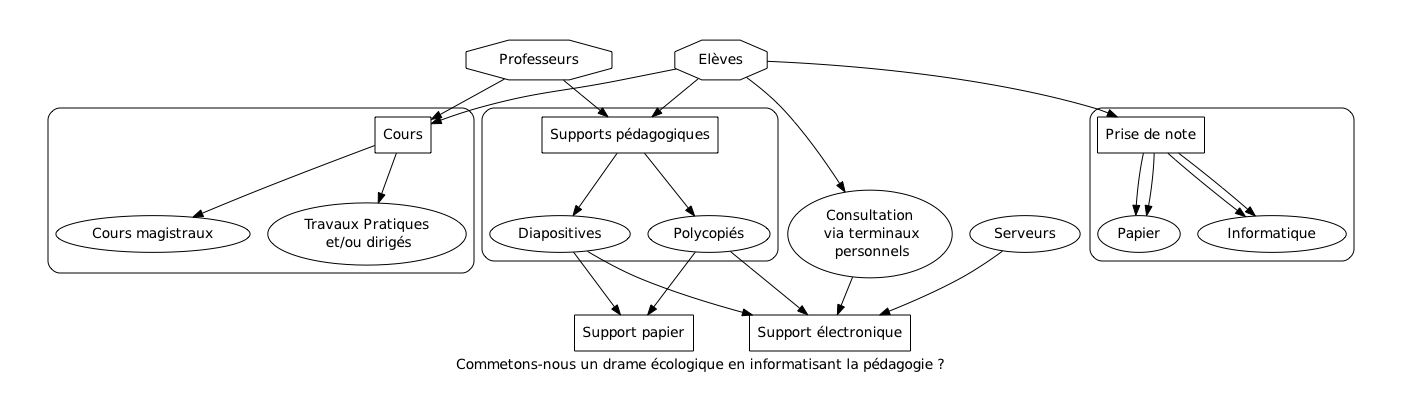
\includegraphics[width=\textwidth]{graphe.png}
\caption{Graphe des relations au matériel électronique}
\label{graphe}
\end{figure}

On y retrouve les professeurs ainsi que les éleves, les cours, les notes prises par les étudiants et les supports pédagogiques. Ces divers éléments ont une seule raison d'être : mettre en évidence les changements que la pédagogie française a subi ces dernières années en terme informatique : les professeurs projettent leur cours sur des présentations animées, les élèves prennent des notes sur leur ordinateur portable puis réitère leur utilisation lorsqu'il souhaite réviser...\\

Penchons-nous de plus près sur les différentes problématiques :

\subsubsection{Les professeurs}
\begin{enumerate}
\item Nous partirons du constant suivant : les professeurs sont de moins en moins sujets à rédiger des supports de cours dont a forme d'un polycopié qui sera édité et distribué à l'ensemble des élèves; mais plutôt sous la forme de diapositives qui seront projetées par la suite en cours. Il s'agira donc de cerner les habitudes des professeurs, que ce soit en cours magistral ou en travaux dirigés, pour définir le temps passé et/ou gagné à ce changement.
\item Quelles sont leurs habitudes de travail : Impression des sujets de travaux pratiques, projection du cours à l'aide d'un vidéo-projecteur, évaluation des élèves via un serveur de centralisation... Tous ces points pèseront dans l'utilisation que l'enseignant et les étudiants feront de leur ordinateur.
\end{enumerate}


\subsubsection{Les élèves}
\begin{enumerate}
\item De plus en plus d'élèves utilisent un ordinateur portable pour prendre en note le cours qu'ils suivent. Cette pratique semble se répandre non seulement dans le groupe des Élèves-Ingénieurs en Informatique de troisième année, mais aussi dans l'ensemble de la promotion à l'Ecole Centrale de Nantes.
\item Quel est leur comportement face aux slides projetées/distribuées par les professeurs ? Il est à noter que certains voire plusieurs élèves imprimeraient l'ensemble des diapositives du cours afin de pouvoir les travailler sur un support papier.. Ces pratiques sont à cerner pour le bon déroulement de cette étude.
\item Existe-t-il une préférence entre le format électronique et celui papier pour réviser/revoir le cours ? Quels terminaux utilisent-ils (ordinateurs portables, ordinateurs de bureau, smartphones)?
\item Enfin, une question qui s'éloigne du 'développement durable' mais dont la réponse n'est pas dénuée d'intérêt : quel impact pour leur attention en cours, leur performance de révision ?
\end{enumerate}

\subsubsection{Les infrastructures et matériels}
Brièvement, définissons ici les divers outils informatiques liés à la 'cyberpédagogie'. 
\begin{enumerate}
\item Les serveurs: Combien sont-ils ? Quels sont leur consommation ? Quel impact écologique de leur livraison? Quel amortissement ?
\item Les ordinateurs de l'Ecole et des élèves: Quels types ? Quelle consommation ? Quel amortissement ?
\item Le papier en tant que vieux support: à titre comparatif, une étude similaire mais d'un point de vue 'papier-stylo' doit être réalisé afin de mettre en exergue les avantages ou les inconvénients des ordinateurs dans les salles de cours.
\end{enumerate}


Comme annoncé lors du précédent article, nous avons choisi d’étudier les différents usages de l’informatique à l’École Centrale de Nantes. Nous avons tout d’abord interrogé le Centre des Ressources Informatiques de l’école. Cependant, devant l’ampleur de la tâche, notamment la prise en compte de tout le matériel réseau, des onduleurs,etc… Nous avons estimé que nous dépassions largement le cadre d’un simple article de blog.

\section{\'Eleves}
Nous avons créé des questionnaires à l’attention des professeurs ainsi qu’à celle des élèves. Nous allons traiter dans cette section le questionnaire pour les élèves, qui nous a donné entière satisfaction puisque plus de 330 étudiants y ont répondu. C’est donc des données représentatives que nous avons la chance de traiter et que nous allons tenter d’analyser.\\

La première question (\textit{c.f.} figure~\vref{i1}) concernait le nombre d’ordinateurs portables. Une très grande majorité d’entre nous possède un et un seul ordinateur portable ($90\%$). Ce résultat, même dans une école d’ingénieurs, reflète la démocratisation des solutions informatiques portables et l’essor du portable qui bat désormais en nombre de vente les ordinateurs dits fixes.\\

\begin{figure}[h!]
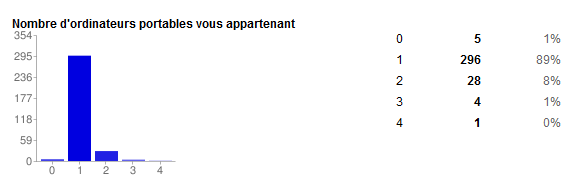
\includegraphics[width=\textwidth]{i1.PNG}
\caption{Question 1}
\label{i1}
\end{figure}

La seconde question (\textit{c.f.} figure~\vref{i2}) concernait le rapport des élèves aux diapositives pendant les révisions. En effet, avant l’école la plupart d’entre nous n’étions pas familiers avec les présentations, notamment en prépa où le tableau est le plus souvent utilisé. La moitié des élèves sont plutôt ou très enthousiastes concernant le rôle des diapositives. Un quart estime que leur rôle est nul et enfin, un dernier quart juge leur influence néfaste.\\

\begin{figure}[h!]
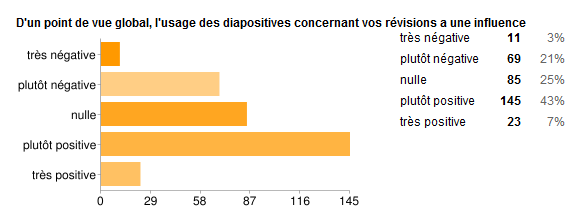
\includegraphics[width=\textwidth]{i2.PNG}
\caption{Question 2}
\label{i2}
\end{figure}


De façon surprenante, surtout pour les élèves de l’option Informatique, seulement $14\%$ des élèves suivent les cours à l’aide de leur ordinateur (\textit{c.f.} figure~\vref{i3}). $40\%$ de façon occasionnelle et enfin $46\%$ ne suivent jamais les cours avec leur ordinateur. Voici, donc une information importante : ils semblent donc que leur ordinateur soit plus un outil de loisir ou de travail personnel que réellement un outil utile au support pédagogique.

\begin{figure}[h!]
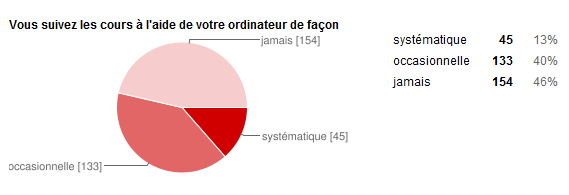
\includegraphics[width=\textwidth]{i3.PNG}
\caption{Question 3}
\label{i3}
\end{figure}


Une question cruciale pour l’informatique verte était de connaître le comportement des élèves vis-à-vis de l’impression des cours (\textit{c.f.} figure~\vref{i3}). Assez logiquement, les $dfrac{3}{4}$ des élèves n’impriment rien, $dfrac{1}{5}$ des élèves impriment certaines pages ciblés et enfin moins de $10\%$ imprime leur cours intégralement.

\begin{figure}[h!]
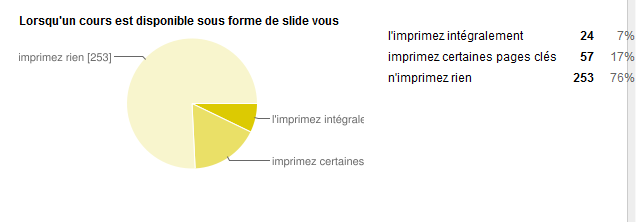
\includegraphics[width=\textwidth]{i4.PNG}
\caption{Question 4}
\label{i4}
\end{figure}


Enfin, le support papier reste le format le plus apprécié pour les révisions, plébiscité par plus de $85\%$ des élèves (\textit{c.f.} figure~\vref{i3}).


\begin{figure}[h!]
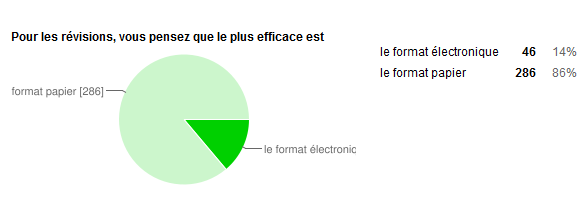
\includegraphics[width=\textwidth]{i5.PNG}
\caption{Question 5}
\label{i5}
\end{figure}


En croisant les différentes données obtenues nous pouvons aller plus loin dans notre analyse. Ceux qui trouvent que les diapositives ont une influence très négative ou négative préfèrent logiquement le support papier à plus de $95\%$. De même les personnes trouvant que les diapositives ont une influence positive ou très positive utilisent légèrement plus que la moyenne l’outil informatique pour suivre les cours de façon systématique $18\%$. Les résultats pour les personnes trouvant que les diapositives n’ont pas d’influence sont eux aussi très homogènes. La perception des diapositives concernant les révisions semblent indépendantes de leurs préférences d’impression ou de suivi de cours.\\

On peut enfin noter que les personnes suivant les cours de façon systématique avec leur ordinateur sont plus nombreuses que la moyenne à préférer le support électronique au format papier $38\%$ contre $15\%$ en général.\\

Nous tenons une fois de plus à remercier le CRI pour avoir répondu à nos questions, ainsi que les élèves ayant pris le temps de répondre à notre questionnaire.


\section{Les enseignants}
Qu'en est-il de l'utilisation de l'informatique pour les enseignants de l'Ecole Centrale de Nantes ? Leur démarche est-elle écologique ?\\

Cette section décrit les résultats issus des réponses de près de 55 enseignants de l'Ecole Centrale.

\subsection{Questions d'ordre général}

\subsubsection{L’utilisation des ordinateurs par les enseignants}

Dans un premier temps, nous pouvons nous questionner sur l'utilisation des ordinateurs d'un point de vue global. Combien de temps celui-ci est utilisé par jour ? Voilà une première question qui peut nous permettre une prise de conscience cruciale dans la suite de notre étude.\\

Il convient de distinguer deux cas :
\begin{itemize}
\item Premier cas : l'utilisation de l'ordinateur dans l'enceinte de l'Ecole Centrale, que ce soit pour une activité d'enseignement directe (lors de cours) ou indirecte (préparation des cours, des TD, correction de divers travaux, etc) \textit{c.f.} figure~\vref{i3}
\item Deuxième cas : l'utilisation de l'ordinateur chez l'enseignant en préparation des cours \textit{c.f.} figure~\vref{i3}
\end{itemize}

\begin{figure}[h!]
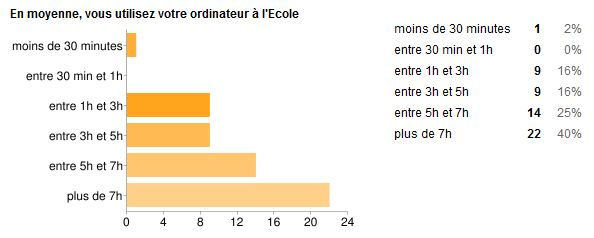
\includegraphics[width=\textwidth]{i6.PNG}
\caption{Question 1}
\label{i6}
\end{figure}

\begin{figure}[h!]
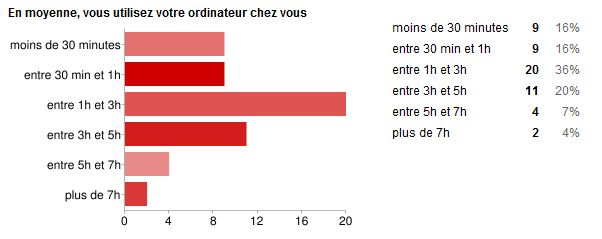
\includegraphics[width=\textwidth]{i7.JPG}
\caption{Question 2}
\label{i7}
\end{figure}

Cette séparation nous permet de mettre en évidance que la grande majorité des enseignants utilise de manière quasi-continue leur ordinateur au sein de l'Ecole Centrale de Nantes. Il s'agit de prendre en compte l'impact électrique de ces ordinateurs sur le réseau de l'école.\\

De même, nous remarquons que l'enseignant utilse l'outil informatique de manière soutenue puisque $36\%$ d'entre eux l'allume chez eux entre 1h et 3h pour préparer les cours, et de même $20\%$ d'entre eux entre 3h et 5h.\\

Soit dit en passant, une analyse croisée-dynamique nous permet d'établir la moyenne d'utilsation des ordinateurs par les enseignants à prés de 8h15mn par journée de travail. En référence à l'article précédent, notamment cet outil, nous pouvons approcher le coût électrique par enseignant à 50,6\euro{} par an.\\

\paragraph{Caractéristique de la simulation}

\subparagraph{Temps d'utilsation :} 8,28 heures par jour.
\subparagraph{Consommation en Watt (W) de l'appareil :}250 W.
\subparagraph{Prix du kilowattheure :} 0.097\euro{}. 

\paragraph{Détail du calcul}

1 kilowattheure vaut 3 600 000 Joules (J).\\
La durée moyenne d'utilisation par jour est 29808 secondes (s).\\
La consommation d'énergie pendant une journée d'utilisation vaut 7452000 J.\\

\begin{center}
\begin{tabular}{|c|c|}
\hline  Energie (J)	& Prix (\euro{})  \\ 
\hline  3600000 &  0,097\\ 
\hline  7452000 & ? \\ 
\hline 
\end{tabular} 
\end{center}

En une journée, cela équivaut à environ 0,2\euro{} par jour.\\

En comptant une année à 253 jours ouvrés, l'année 2011 coûtera 50,6\euro{} par enseignant et par an à l'Ecole Centrale de Nantes. ce qui est, avouons-le, relativement peu pour l'utilisation intensive qu'ils en font.\\



\subsection{Etude énergétique plus approfondie}

Certes, je conviens que le résultat précédent n'est qu'une approximation du coût réel. Il repose sur l'hypothèse selon laquelle les ordinateurs portables sont sur le secteur tout au long de leur utilisation, et ont une consommation de 250W (consommation d'un MacBook Pro dual core).\\

Pour affiner cette étude, il s'agit d'établir d'une manière plus précise comment se structue le parc informatique des enseignants de l'Ecole Centrale de Nantes. Pour cela, les questions suivantes vont nous éclairer. Faisons quelques remarques rapides et rétablissons notre calcul (\textit{c.f.} figure~\vref{i8}).\\

\begin{figure}[h!]
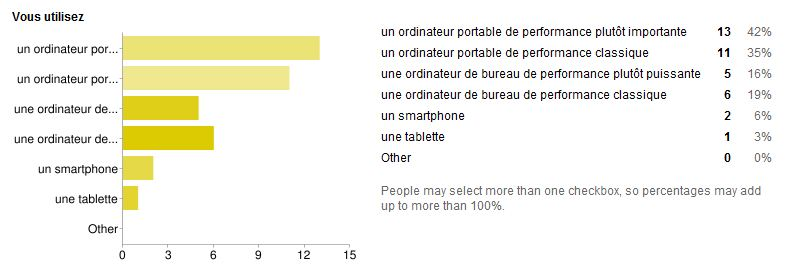
\includegraphics[width=\textwidth]{i8.JPG}
\caption{Question 3}
\label{i8}
\end{figure}

\begin{itemize}
\item Le parc informatique correspond à un parc de machines portables plutôt puissantes
  \begin{itemize}
  \item $42\%$ de portables de haute performance : gardons 250W qui est une bonne référence en parcourant les différents constructeurs.
  \item $35\%$ de portables de performace classique: prenons 125W qui représente la moitié de cette consommation.  
  \end{itemize} 
\item Et deux fois moins d'ordinateurs de bureau (consomment $50\%$ à $80\%$ en plus qu'un ordinateur protable [notamment à cause de l'écran], disons $65\%$)
  \begin{itemize}
  \item $16\%$ de PC de haute performance: 162W
  \item $19\%$ de PC de performance classique: 81W
  \end{itemize} 
\end{itemize}

Ce qui réduit la consommation moyenne d'un ordinateur à \textbf{170W}.\\
\begin{center}
\textbf{En conclusion, nous arrivons à un total de 38,2\euro{} par enseignant par an.}
\end{center}

\begin{figure}[h!]
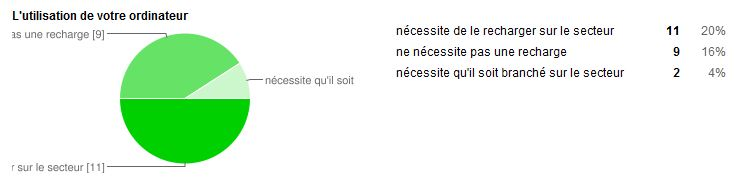
\includegraphics[width=\textwidth]{i9.JPG}
\caption{Question 4}
\label{i9}
\end{figure}

\begin{figure}[h!]
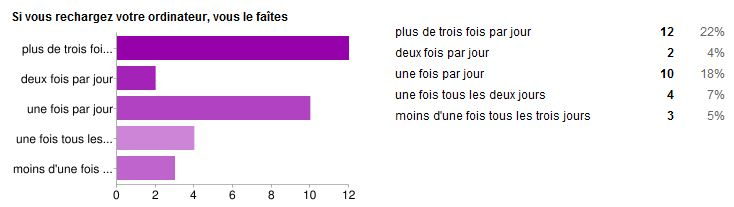
\includegraphics[width=\textwidth]{i10.JPG}
\caption{Question 5}
\label{i10}
\end{figure}


\paragraph{Remarque}
Il est utile de noter que $16\%$ des usagers disent ne pas avoir besoin de recharger ler portable sur le campus. Il convient que cette charge ne sera pas à prendre pour le compte de l'Ecole; mais étant donnée que nous effectuons une étude sur l'impact général de l'informatique dans la pédagogie, nous ne prendrons pas ce résutlat en compte (la recharge arrivera bien à un moment donné, que ce soit chez eux ou à l'école).\\


\subsection[Quelles suprématies ?]{La suprématie des présentations via diapositives, mais le maintien des habitudes papier}

Passons maintenant aux problémtiques liées au cours lui-même (\textit{c.f.} figure~\vref{i11}).\\

\begin{figure}[h!]
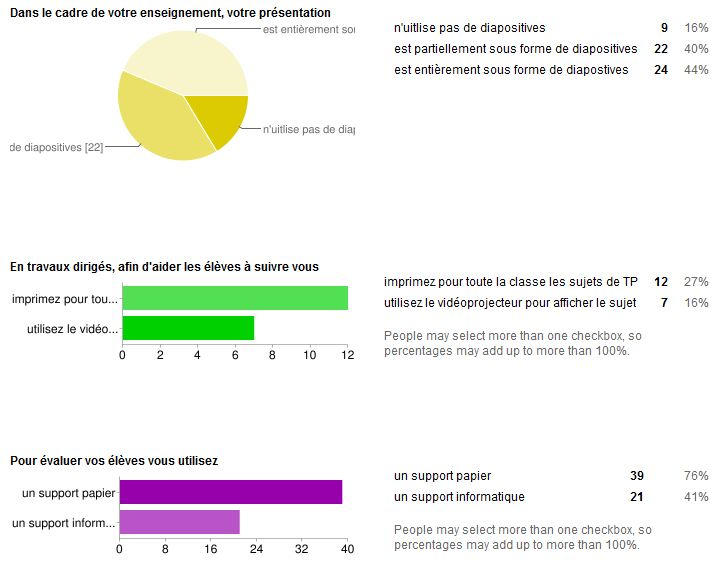
\includegraphics[width=\textwidth]{i11.JPG}
\caption{Question 6}
\label{i11}
\end{figure}

Les résultats correspondent aux idées reçues du moment : s'appuyer sur des diapositives pour illustrer ses propos est désormais quasi-incontournables. En effet, près de $84\%$ des enseignants disent utiliser des diapositives, dont $44\%$ les utilisent pour la totalité de leur cours.\\

Néanmoins, il s'agit de garder à l'esprit les problématiques suivantes :

\paragraph{Tous les élèves n'ont pas un ordinateur.}
Ce fait est un droit, et ne doit pas se transformer en un devoir de possession d'un tel outil. Comment justifier de l'achat d'une machine qui équivaut quasiment à un loyer étudiant ? Malgré eux, les élèves sont pratiquement obligés de faire acquisition d'une machine personnelle, même si des ordinateurs sont à la disposition de tous.\\

En effet, il est pénible, comme le montre l'étude précédente, de devoir imprimer l'ensemble des présentations (plus de 100 pages en moyenne) alors qu'elles ne se prêtent pas du tout à ce but (difficulté de mise ne page, difficulté de compréhension du fait de la concision de celles-ci, etc).\\

Les élèves préfèrent parcourir les diapositives lors de leur révision. A part envisager des révisions en salle informatique (souvent bruyantes), les élèves se doivent d'avoir une ordinateur personnel...\\

\paragraph{Il est techniquement difficile d'évaluer les élèves pour un moyen informatique}
Sauvegarde et accès aux données, problèmes de tricherie (utilisation des moyens de communication externes, et recherches sur la toile) et équipements adéquats (en qualité et surtout en nombre) sont autant de problèmes se dressant devant l'évaluation sur un support informatique.\\

Il est important de mettre la lumière sur les résultats de la question "Pour évaluer vos élèves vous utilisez" dont beaucoup d'enseignants ($41\%$) ont répondu le support informatique.\\

Je ne les remets pas en cause ; ils sont d'autant plus vrais qu'ils deviennent un standard dans la vie quatidienne des élèves. Cependant n'oublions pas de préciser que ces évaluations sont inscrites dans le cadre de travaux pratiques ou de travaus à la maison, qu'il faut rendre, avant une date limite, au professeur concerné en lui envoyant par mail une version pdf du travail (ou en utilisant le logiciel libre Markus depuis peu pour les matières informatiques de l'Ecole Centrale de Nantes [ici plus d'articles sur EAT-TICE Centrale Nantes])\\



\subsection{Avis global des enseignants}

Pour finir, les résultats suivants permettent d'avoir une vision générale des questionnements sur l'informatique verte au sein de la communauté des enseignants (\textit{c.f.} figure~\vref{i12} et figure~\vref{i13}).\\

\begin{figure}[h!]
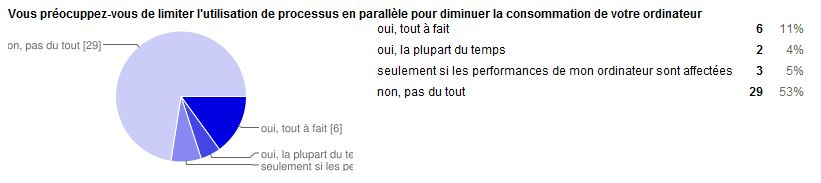
\includegraphics[width=\textwidth]{i12.JPG}
\caption{Question 7}
\label{i12}
\end{figure}

\begin{figure}[h!]
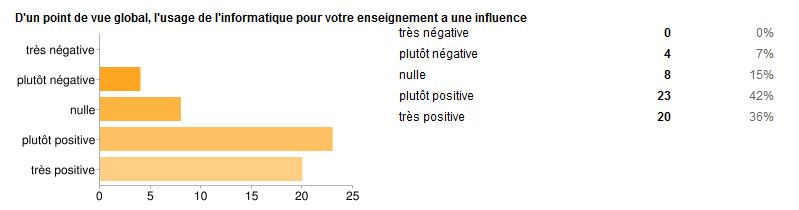
\includegraphics[width=\textwidth]{i13.JPG}
\caption{Question 8}
\label{i13}
\end{figure}


C'est un fait, une très grande part des enseignants utilisentn leur ordinateur sans se soucier des consommations électriques qu'ils engendrent. Nous pouvons effectuer deux remarques :\\
\begin{itemize}
\item Nous avons montré dans cette étude que l'utilisation des ordinateurs est clairement répandue chez les enseignants. Chaque professeur disposant d'un ordinateurs personnel, leur nombre ne devrait pas varier pour une population fixe. De plus, si aucun effort particulier n'est fait par les utilisateurs pour réduire leur consommation électrique, il est très probable qu'une campagne de sensibilisation permette d'obtenir des résultats positifs (au pire ils stagnent). Enfin, les ordinateurs diminuent porgressivement leur consommation électrique tout en augmentant leur performance; quand bien même les enseignants changeraient de machines dans quelques années, il est fort problable que leur consommations soient identiques à caujourd'hui. Aussi, nous pouvons conclure que la consommation électrique du parc informatique de l'Ecole Centrale de Nantes ne pourra que baisser dans le futur (sauf augmentation du nombre d'enseignants ie. d'élèves, ce qui est fort probable).
\item Enfin, une très grande majorité des enseignants considèrent l'outil informatique comme clairement positif dans la pédagogie. Pour un coût électrique faible, les avantages semblent bien plus important que l'impact de consommation électrique qu'ils engendrent.. N'oublions pas néanmoins qu'un ordinateur "coûte du carbone" à sa conception, production, réparation et recyclage... Qui sait, peut-être qu'un prochain article décrira ce grand autre sujet !
\end{itemize}

Je remercie les enseignants d'avoir participé à ce questionnaire en consacrant un peu de leur temps pour que je puisse rédiger cet article.


\newpage
\part{Pour aller plus loin...}
\section{Calcul générique sur un processeur graphique}
\subsection{Généralisation des solutions de calculs basées sur les processeurs graphiques}
Comme l’a encore montré le dernier classement\footnote{\textsf{http://www.top500.org/list/2010/11/100}} des plus puissants supercalculateurs, la demande croissante en calcul nécessite de trouver de nouvelles solutions. Depuis quelques années, l’utilisation de GPU\footnote{\textsf{http://fr.wikipedia.org/wiki/Processeur\_{}graphique}} s’est généralisée : 3 des 5 premiers utilisent des solutions basées sur des GPU Nvidia. Ceci s’explique principalement par la très forte parallélisation des calculs, rendue possible grâce aux nombreux cœurs. Il s’agit d’une situation de co-traitement : les parties séquentielles sont traitées par les CPU tandis que les parties demandant le plus de calculs sont traitées par le GPU, cela s’appelle le GPGPU\footnote{\textsf{http://fr.wikipedia.org/wiki/General-Purpose\_{}Processing\_{}on\_{}Graphics\_{}Processing\_{}Units}} (General-Purpose Processings on Graphic Units).\\

\subsection{Intérêts des processeurs graphiques dans le cadre de l'informatique verte}
L'utilisation de GPU concernant les calculs nécessitant beaucoup de ressources possède un autre avantage, particulièrement importante pour l'informatique verte. Elle réduit considérablement la puissance de calcul par Watt. On peut à ce titre consulter la Green List\footnote{\textsf{http://www.green500.org/lists/2010/11/top/list.php}}. Ce classement montre encore plus l’efficacité énergétique d’une solution basée sur les GPU et le rôle de plus en plus important qu'il joue dans les calculs scientifiques. On peut notamment constater que la plupart des projets utilisant BOINC, et notamment les plus connus tels que Seti@Home ou Folding@Home propose des versions utilisant les ressources des processeurs graphiques afin d'abaisser les temps de calcul.\\

On remarquera de plus qu’une telle approche réduit considérablement les coûts. Ainsi, en décembre 2010, le téraflops\footnote{\textsf{http://fr.wikipedia.org/wiki/FLOPS}} en simple précision coûte 1000\euro{}  soit approximativement 10 fois moins qu’une solution équivalente basée sur des CPU.\\

Ce domaine très spécifique, de l'utilisation de GPU pour les calculs facilement parallélisables, va vraisemblablement s’intensifier et Nvidia prévoit des GPU de 20 teraflops en double précision avant 2020\footnote{\textsf{http://www.presence-pc.com/actualite/Echelon-41475/}}.\\

Une structure telle qu’une école d’ingénieurs serait ainsi l’environnement idéal pour déployer un tel système. Les GPU permettent une consommation énergétique réduite à puissance de calcul égale. Ils sont de plus attractifs que ce soit en coût à l’achat, qu’en coût de fonctionnement.\\

\subsection{Inconvénients de telles solutions}
Un frein majeur à un tel déploiement reste cependant la programmation exploitant de tels ressources. En effet, l'utilisation massive de GPU étant assez récente les langages permettant d'en tirer partie sont encore peu connus. On en dénombre pour le moment trois principaux : CUDA\footnote{\textsf{http://www.nvidia.fr/object/cuda\_{}home\_{}new\_{}fr.html}} pour Nvidia, ATI Stream\footnote{\textsf{http://www.amd.com/US/PRODUCTS/TECHNOLOGIES/STREAM-TECHNOLOGY/Pages/stream-technology.aspx}} pour ATI et OpenCL\footnote{\textsf{http://www.khronos.org/opencl/}}, à l'origine développé par Apple et qui semble se dégager comme une alternative intéressante.\\

Pour conclure, le GPGPU possède d'indéniables avantages : une puissance de calcul très importante pour une consommation énergétique et un coût réduits. Cependant, son évolution rapide nécessite de la part d'universitaires soucieux de faire bénéficier de serveurs de calcul puissants, du temps et des connaissances nouvelles pour assurer la mise en place d'une telle structure.\\




\section[\'Etude d'un livre]{\'Etude du livre : \og Green IT : Gérez la consommation d'énergie de vos systèmes informatiques \fg}

Cet article sera intégralement dédié à la présentation du livre \underline{Green IT : Gérez la consommation d'énergie de vos systèmes informatiques} d’Olivier PHILIPPOT. Il constitue un bref résumé de son contenu et nous ne pouvons que vous encouragez à en faire l’acquisition pour approfondir le sujet.\\

\subsection{Situation actuelle de la consommation électrique dûe à l'informatique}
En 2009, selon le rapport DETIC\footnote{\textsf{http://lesrapports.ladocumentationfrancaise.fr/BRP/094000424/0000.pdf}}, les technologies de l’information et de la communication ont consommé 60 TWh, représentant $13,5\%$ de la facture électrique française. De plus, cette consommation croît très fortement et pose un problème écologique majeur, lié à la production de l’énergie nécessaire.\\

Les rapports Meadows (1972 - traduit en français par \og Halte à la croissance \fg \footnote{\textsf{http://fr.wikipedia.org/wiki/Halte\_{}\%C3\%A0\_{}la\_{}croissance\_{}\%3F}}) et Facteur 4 (1996) du Club de Rome proposent une solution simple : réduire la consommation d’énergie. Il est en effet plus rentable d’économiser de l’énergie que de la produire. Par exemple, 1 kWh informatique utile économisé sur un ordinateur, c’est de 15 à 60 kWh d’énergie primaire.\\

La première façon de mettre fin au gaspillage est de dimensionner convenablement le parc informatique. Bien souvent, les ordinateurs restent allumés de façon constante sans être utilisés, tout comme les imprimantes (il est facile de s’en rendre compte à Centrale). Selon une étude\footnote{\textsf{http://www.enertech.fr/docs/R\_{}FinTIE50.pdf}} Enertech pour l’ADEME, sur la totalité des imprimantes laser auditées, plus de $60\%$ sont toujours activées. De surcroît, beaucoup de sociétés laissent tourner leur parc informatique la nuit et les week-ends comme l’a montré une étude faite en 2004 (After-hours Power Status of Office Equipment and Inventory of Miscellaneous Plug-Load Equipment - Berkeley National Laboratory - Janvier 2004).\\

Un autre point à prendre en compte et plus surprenant est la consommation importante lorsque l’ordinateur est éteint mais toujours branché : elle est en moyenne de 117 kWh/an. (Étude Enertech pour l’ADEME vue précédemment).

\subsection{Mesures à mettre en place}
Le principal frein aux avancées dans le domaine de l’informatique verte est bien entendu l’utilisateur : habitudes, mauvaise compréhension des architectures réseaux ou de l’ordinateur sont autant de points qui empêchent la mise en place d’une gestion cohérente des économies d’énergie. Au niveau supérieur, les sociétés sont également responsables en ne sensibilisant pas assez leurs employés sur les moyens pourtant simples pour aider l’entreprise à alléger sa facture énergétique. Enfin, pour une réelle efficacité, les gouvernement doivent mettre en place des mesures visant à favoriser les comportements « verts » en mettant à disposition des documents et en encourageant les entreprises par la perspective des réductions des factures d’électricité. Cet élément jouera un rôle d’autant plus conséquent, au vue des hausses annoncées des prix de l’énergie pour les années à venir.\\

\subsection{Moyens de réduction de la consommation électrique}
De nombreuses méthodes sont disponibles pour réduire la consommation électrique. Ainsi, le renouvellement du parc informatique s’il est possible et pertinent (il s’agit de prendre en compte également le recyclage du matériel usagé) et grâce à l’évolution des systèmes d’exploitation aussi bien que des processeurs sont des moyens d’action liés aux avancées technologiques. Des logiciels sont également à disposition et permettent de réduire de façon conséquente la consommation de l’équipement informatique.\\

Afin de répondre au mieux au besoin, des entretiens ou des sondages comme nous en avons menés lors des articles précédents peuvent permettre de connaître au mieux le besoin énergétique réel. Il existe également des sociétés spécialisées dans l’audit énergétique telles que Terra Nova, Aergy ou Neoditel.\\

Si cela est trop complexe ou trop coûteux, un inventaire complet du parc informatique, associé à une grille de consommation moyenne ou des formules disponibles sur Internet permettent déjà d’avoir une idée assez juste de la situation. Afin d’ajouter de la précision au calcul tout en maintenant des coûts d’études réduits, on peut installer des wattmètres qui vont mesurer la puissance consommée par le matériel.\\

L’auteur préconise alors la mise en place d’une politique énergétique, expliquant le but de l’action tout en restant simple, succincte et cherchant à impliquer au maximum l’utilisateur final au processus d’économie d’énergie. Ainsi, une telle politique a été mise en place chez Vodafone en Grèce et a permis d’économiser 1 million d’euros sur la facture énergétique (pas seulement informatique). En France, l’État met en place des actions et des aides pour le PME pour soutenir l’informatique verte. Ces actions seront d’autant efficaces que l’on pourra évaluer les gains potentiels.\\

En conclusion, les utilisateurs n’ont pas encore pour la plupart des comportements conformes à l’informatique verte. Dans le passé, cela était principalement lié à des contraintes technologiques et organisationnelles, mais les progrès constatés ne justifient plus une telle aberration. Les sociétés doivent ainsi réaliser un inventaire associé à un audit des consommations. Elles pourront alors estimer les gains réalisables et mettre en place une politique énergétique. Dans l’idéal un responsable ou une équipe entière seront dédiés à l’informatique verte dans l’entreprise.\\



\section[Réduire sa consommation]{Réduire la consommation électrique de votre ordinateur}

Ecouter la musique, lire ses mails, rédiger un rapport et consulter ses flux RSS. Voilà un bref aperçu des activités que nous faisons naturellement chaque jour grâce à notre ordinateur. Avez-vous déjà pensé combien cela peut-il vous coûter ?
Certes un ordinateur consomme peu d'électrcité en comparaison d'un chauffage électrique, mais entre votre écran, l'imprimante, les disques durs interne et externes, votre routeur wifi, etc, voilà déjà une foule de gourmands électriques prêts à sévir sur votre facture EDF...\\

Ne paniquez pas! Nous vous proposons de parcourir cette section qui présentet les principaux axes de solutions, et de suivre les conseils qui y sont décrits.\\
\begin{center}
\emph{La nature (et votre porte-feuille) vous remercieront.}
\end{center}

\subsection{La consommation d'un ordinateur}

\subsubsection{Généralités}
D'après ConsommerDurable.com\footnote{\textsf{http://www.consommerdurable.com/2010/08/comment-reduire-sa-consommation-d-energie-et-sa-facture-d-electricite/}}, la consommation annuelle moyenne d’électricité d’un ordinateur est de 219 kWh/an ce qui représente un coût de 25 euros par poste informatique. Mais ce chiffre varie d’une manière importante en fonction du type d’appareil et de l’utilisation qui en est faite. Ainsi, un ordinateur qui fonctionne 24h/24h peut engendrer une dépense annuelle d’électricité de plus de 100 euros. Pour limiter la consommation d’énergie engendrée par les équipements informatiques :

\paragraph{Privilégiez l’utilisation des ordinateurs portables}
En moyenne, un ordinateur portable consomme 50 à 80% d’énergie en moins qu’un ordinateur fixe muni de son écran.

\paragraph{Activez les fonctions \og économies d’énergie \fg}
Le premier intéressé, EDF, estime quant à elle à \textbf{12,74 euros par an} le coût moyen en électricité d'un micro-ordinateur. Ce montant est trois fois supérieur à celui d'un sèche-cheveux, et représente pratiquement le double de celui d'une chaîne hi-fi [source 01.net].\\

Comme vous pouvez le remarquern, les deux sources présentées ici ne donnent pas la même valeur pour le coût induit par un ordianteur. cela est principalement dû aux différences matérielles entre les différents ordinateurs. N'oublions pas qu'un EeePc consommera moins qu'in ordinateur de bureau !\\

En parcourant la toile, j'ai trouvé un petit simulateur\footnote{\textsf{http://biotrans.free.fr/?/aquarium/p-calcul\_{}cout/calcul-cout-consommation-electrique-euro-watt.htm}} qui pourrait vous intéresser. Il permet, connaissant la consommation en Watt d'un appareil, d'en calculer le coût par jour.\\

Mais vous allez me dire : "Comment connaitre la consommation électrique de MON ordinateur?". Rien de plus simple, le site \textsf{http://poloastucien.free.fr/alim\_{}calcul\_{}h.html} permet de se faire une idée de la consommation en Watt de chaque composant!

En faisant le test pour mon ordinateur, je m'aperçois que mon ordinateur me coûte (au minimum) 54 euros par an. Pourquoi au minimum ? Parce que j'ai un double écran, des basses sur lesquelles tournent très souvent de la musique, plus ma lampe de bureau pour ne pas avoir mal aux yeux...\\

Faîtes le test!

\subsubsection{Eteindre son ordinateur est primordial}
Tout le monde sait bien qu'il faut éteindre son ordinateur lorsque nous ne l'utilisons pas, ou bien le mettre en veille dans le cas si on doit l'utiliser plusieurs fois dans une même journée.\\
Il est important de préciser qu'\textbf{éteindre son ordinateur n'endomage pas le système}, bien au contraire ! D'après ETCY, la défaillance du disque dur est attribuable à la fatigue du bras de lecture provoquée par les lectures et les écritures répétées et non pas aux démarrages. Si l'on se fie aux spécifications des fabricants, les disques durs actuels peuvent démarrer de 10 000 à 50 000 fois avant que des problèmes ne surviennent. Or, si l'on met l'ordinateur en marche cinq fois par semaine, le dix millième démarrage ne surviendra qu'après 38 ans! Votre appareil sera alors désuet depuis belle lurette. De plus, comme la durée de vie moyenne d'un disque dur est de 25000 heures, éteindre l'ordinateur permet de le garder plus longtemps, lui aussi.\\

Il est donc formtement conseiller d'éteindre son ordinateur dès que l'occasion se présente (plus d'une heure sans utilisation), et de n'utiliser sous aucun prétexte les économisateurs d'écrans qui n'ont d'économe que leur nom.



\subsubsection{Outils permettant d'optimiser sa consommation}
\paragraph{Sous Windows\copyright}

Deux logiciels permettent de gérer la consommation de son ordinateur.
\begin{enumerate}
\item Le logiciel Local Cooling, logiciel gratuit qui, une fois installé sur votre PC, va configurer ce dernier pour réduire au maximum sa consommation d'énergie : arrêt de l'écran au bout d'un certain temps d'inactivité, puis des disques durs, et éventuellement même du PC. Il permet de savoir ce que l'on a économisé grace aux modifications de la configuration.
\item Le logiciel Edison, pemet de faire des éconmies d'énergies en contrôlant le comportement de votre ordinateur. Un paramétrage de celui-ci permet une mise en veille et une extinction programmée sur les pages hoaraires définies.
Vous pouvez suivre sur PCAstuces.com, un tutoriel pour réduire la consommation électrique de votre PC, en utilisant notamment le logiciel Local Colling présenté ci-dessus. Il décrit ensuite les paramètres du Panneau de Configuration adéquats pour gérer la mise en veille de celui-ci.
\end{enumerate}

\paragraph{Sous GNU/Linux}
Deux principaux outils :

\begin{enumerate}
\item Tout d'abord PowerTop d'Intel, qui a eu l'idée de créer un outil d'analyse de la consommation d'énergie des logiciels tournant sur le système GNU/Linux et sur une plateforme Intel. (une explication en français de PowerTop)
\item Puis laptop-mode, mais qui pourrait user prématurément le disque dur...
Vous pouvez consulter lesswatt.org, qui est un site anglophone sur l'optimsation de la consommation électrique sous linux.
\end{enumerate}

\paragraph{Sous MacOS\copyright}
Il existe un calculateur d'économie d'énergie si vous utilisez les préférences système...



\subsection{Les conseils à suivre}
En plus de configurer correctement son ordinateur pour économiser de l'énergie, c'est surtout en effectuant quotidiennement certains gestes que vous réduirez votre consommation d'énergie.\\

\paragraph{Nos conseils}
\begin{enumerate}
\item Eteignez vos hauts parleurs lorsque ceux-ci ne fonctionnent pas.
\item Eteignez votre imprimante entre chaque travail d'impression.
\item Eteignez l'écran lorsque vous quittez temporairement votre ordinateur.
\item Eteignez votre ordinateur ou mettez-le en veille lorsque vous quittez plus de 30 minutes votre ordinateur.
\item Même en veille, un appareil électrique consomme de l'énergie. Une prise multiple peut vous permettre de débrancher facilement l'ensemble de votre matériel.
\item Préférez un ordinateur portable à un ordinateur de Bureau.
\item Eteignez votre modem / box Internet la nuit.
\end{enumerate}

Vous l'aurez compris, l'idée est simple : tout appareil en veille consomme de l'énergie! Eteignez-les si vous ne les utilisez pas!
En espérant que ces conseils vous auront été utiles !

\newpage
\section{Synthèse}

Tout d'abord, nous avons montré à quel point le lien entre l'informatique et l'écologie s'était intensifié au cours des années. A tel point, qu'il nous est apparu que ces deux domaines sont aujourd'hui indissociable. 
Ensuite et afin d'apporter une réelle plus-value à notre travail et ne pas nous borner à accumuler des données glanées sur Internet, nous avons mené une enquête au sein de l\'Ecole, qui avait pour étude le comportement des élèves mais aussi des professeurs. Elle a permis de mettre en relief certaines habitudes et certains comportements, qui à notre connaissance n'avait pas été étudiés auparavant.
Enfin, nous avons montré différentes solutions pouvant s'appliquer de façon plus générale et à différentes échelles : celle des supercalculateurs avec le calcul par des processeurs graphiques, celle des entreprises (bien que le domaine d'étude de l'ouvrage soit plus vaste) avec l'étude du livre \textbf{Green IT} et enfin celle des particuliers avec des comportements simples.

\section{Conclusion}

A travers cette série d'articles, nous avons cherché à brosser un portrait complet de la situation actuelle de l'informatique verte. Bien entendu, le sujet étant vaste, nous avons donc été contraints de traiter un nombre limité de problèmes.\\
De plus, cette étude ayant pour cadre l'\'Ecole Centrale de Nantes nous avons apporter des solutions pratiques à mettre en place aussi bien pour les professeurs que pour les élèves.

\end{document}
